\section{Introduction}
Technology nowadays tends to adapt to users  \cite{roemmele2016writing:one}\cite{mckee2017professional:two} and exhibiting more human-like affordances such as: social presence \cite{nass1994computers:three} artificial intelligence \cite{mckee2017professional:two}and Autonomous. As remarked by Trip et.al \cite{tripp2011degrees:four}, these are technologies equipped with inbuilt communicative, instructive, and interactive features.
Typical examples are intelligent personal assistance like Google Assistant, Apple Siri, Amazon Alexa and Microsoft Cortana. Or automated homes products (e.g. Google Home and Amazon Echo); or driverless smart cars (e.g. Google Assistant integration with Hyundai).
Typical examples are intelligent personal assistance like Google Assistant, Apple Siri, Amazon Alexa and Microsoft Cortana. Or automated homes products (e.g. Google Home and Amazon Echo); or driverless smart cars (e.g. Google Assistant integration with Hyundai).
These technologies are built to support  human daily activities. for instance,  driving or assist users on daily household  chores (shopping, make an appointment) or even support on small job errands (e.g make a call, send text message)\cite{kamits:five}.
However,  these technologies are faced with problems, such as  low adoption levels \cite{ cowan2017can:six}.  For example Apple Siri is rarely used, evidently in a survey where out of 98\% of Iphone users using Siri, 30\%  uses frequently and 70\% rarely uses \cite{factor1:seven}. This could be associated with many reasons like resistance to change and lack of trust. As there is still a lack of understanding which bring the question of risk on how they operate (e.g. how machine learning algorithm works) and how information is shared (e.g. privacy and ethics) as well as how decisions are made (e.g. autonomous recommendation ).
Aylett et.al \cite{aylett2014none:eight}, believes the problem lies on insufficient users experience studies.  To Trip. et.al \cite{tripp2011degrees:four},  trust is a key element for mitigating the risk associated with the use of human-like technologies.  This vision is supported by Benbasat\& Wang \cite{benbasat2005trust:nine}, who found trust  as an important element in the use of  human-like technology such as online recommendation agents. As well as, Lippert \&Swiercz \cite{lippert2007personal:ten} claims.  
Being aware that trust besides supporting relationships also supports the decision making process when certain amount of risk is associated. As well as can influences the frequency and kind of usage of technical artifacts \cite{nothdurft2013bases:eleven}. We aim towards broaden the understanding of trust and it influence in the adoption of human-like technologies by  exploring how emotions can influence peoples trust in technology. 
As Fine \& Holyfield \cite{fine1996secrecy:twelve} claims there is a need to examine the multidimensionality of trust from dimensions such as emotion amongst others. Basically considering trust as thought and felt. \cite{fine1996secrecy:twelve} (p.25). McAlister \cite{mcallister1995affect:thirteen} describes trust as cognitive and affective classification. In addition, McKnight \& Chervany \cite{mcknight2001trust:fourteen} includes affect (emotion) as  benevolence in their trust model. Also, considering trust conceptualized as behavior by Krammer \cite{kramer1999trust:sixteen} and McKnight \& Chervany \cite{mcknight2001trust:fourteen}. The technology acceptance model (TAM) suggest further that there is interplay between behavior and emotion \cite{tislar2014emotions:seventeen}. We therefore argue that emotions can be linked to the decision making process [\cite{ekman2007emotions:eighteen}\cite{keltner2014sociocultural:twenty}\cite{keltner2010emotion:nineteen}\cite{norman2004emotional:fifteen}] and therefore to trust. 
The appraisal tendency framework (ATF) is a good example  of the study of the influence of emotion on usage of technical artifact and the results suggest that emotion influences usage of technical artifact \cite{beaudry2010other:twentyone}. Also, several researchers [\cite{cristescu2008emotions:twentytwo} \cite{mcgraa2010effects:twentyfive}] suggests that emotions roles are essential to understanding user’s behavior when faced to different application programs.
Since both emotion and trust have proven to be significant indicators for understanding user behavior to enhance technology usage.  We place our efforts on studying the interplay  between emotions affects and users trust when using technologies that exhibit Human like characteristics (i.e.  Social presence, artificial intelligence and Autonomous).
\section{Problem Statement}
Above introduction expresses the need to study trust in technology with Human-like characteristics. As well, as highlighted that trust and emotions are key factors. To understand human behavior towards human-like technology, since persuasion not force or cohesion is needed, to make users change behavior towards technologies \cite{fogg2002persuasive:twentythree}. 
	
Similar to Maes \cite{maes1995agents:fourtytwo},we continue to focus on the problem of trust fostering between users and human-like technologies.  In addition, effort has been made by Yuksel et.al \cite{yuksel2017brains:fourtythree}toward remedying impeding trust problem between users and technologies (intelligent personal assistant), but through understanding the trade-off between physical attractiveness and reliability in technological artifacts. Also, Trip et.al \cite{tripp2011degrees:four} has equally investigated trust issues in human-like technologies using social psychological paradigms.
However, Considering the fact that users trust depends on several factors such as emotion \cite{jones1998experience:fourtyfour} and existence of prior research evidence on the relationship between Emotion and trust in various technological context for example: e-commerce \cite{pelet2013chromatic:twentyseven}, web technologies \cite{kang2012effect:twentyeight} online transactions payment method \cite{tislar2014emotions:twentynine}, formal logic and mathematical modeling \cite{bonnefon2009relation:thirty}.  We focus on fostering trust between users and human-like technologies through unravelling the interplay between emotion and trust of users when interacting with these technologies.
Therefore, the challenge ahead lies on how to foster users trust in human-like technologies through the understanding derived from the interplay between emotion and trust in human-like technologies.  That is to understand the dynamic of these two key factors in foster users willingness to use novel technologies like human-like technologies. Understand and conceptualize the interplay between emotion and trust in human-like technologies. 

Our objective besides focused on unraveling the relationship between trust and emotion during interaction with technical artifacts exhibiting human-like characteristics. Also aims to find such relation from both psychometric and physiological evidence. As well aims to contribute towards developing a conceptual model that maps the various emotions affects to trust in technology with human-like characteristics. 

This outcome beside contributes for system developers, designers, researchers and practitioners in HCI and none HCI field to develop trusted technologies. Support as well further research on developing  emotional intelligence systems that  also foster users trust.

\section{Related Research}
Maes \cite{maes1995agents:fourtytwo} have long pointed out the problem of trust fostering amongst others technologies (intelligent personal assistant). Efforts has been made by several researchers towards fostering trust in these technologies using different approach, for example Yuksel et.al \cite{yuksel2017brains:fourtythree} and  trip et.al \cite{tripp2011degrees:four}. We believe the interplay between emotion and trust is another possible solution to deepen our understanding of users trust in human-like technologies. Considering the fact that users trust depends on several factors notably emotion \cite{jones1998experience:fourtyfour}. Prior research evidence exists proving the relationship between Emotion and trust in various technology contexts except human-like technologies. for example: e-commerce \cite{pelet2013chromatic:twentyseven}, web technologies \cite{kang2012effect:twentyeight} online transactions payment method \cite{tislar2014emotions:twentynine}, formal logic and mathematical modeling \cite{bonnefon2009relation:thirty}. 
Therefore, motivating this research, that aims to foster users trust in technologies with human-like characteristics taking into account the interplay between emotion and trust of users when interacting with humanlike technologies.

\section{Research Question and Hypothesis}
This research is supported mainly by three main conceptualizations. The trust conceptualization that emerges from
Gullathi et.al \cite{gulati2017modelling:twentysix} findings. Where Gullathi et.al \cite{gulati2017modelling:twentysix} describes and assesses the Trust relationship between the user and a technical artifact based on the belief that this technical artifact will exhibit Human Like characteristics. In addition to the McKnight \& Chervany \cite{mcknight2001trust:fourteen} three-dimensional conceptualization view of trust in technology as follows:
\begin{enumerate}
    \item First points1.	Trust intention: the voluntary willingness or subjective probability based on assessment of pros and cons to use a technology
    \item Trust Behavior: the manifestation of the trust intention e.g information sharing, dependence, cooperation with a technical artifact.
    \item Trust believe: the perception of an individual based on cert attributes that they expect a technical artifact to posses or exhibit. 
\end{enumerate}
Another conceptualization to these understanding results from the game theory, a theory also adopted by several researchers when doing trust research [\cite{berg1995trust:thirtytwo},\cite{camerer1988experimental:thritythree},\cite{mccabe2003positive:thirtyfour},\cite{mccabe2000two:thirtyfive}]. This help us to introduce the  risk situation as suggested by Pengnate, \& Sarathy \cite{pengnate2017experimental:thirtyone} where trust represents a key element in the decision process.
The game theory help us also to clearly understand the true user trust intention, behavior and belief when using human like technologies and under various emotional experience. From emotion side we conceptually classify emotion by valence and arousal based on the Geneva emotion wheel version2  \cite{scherer2005emotions:thirtysix},\cite{scherer2013grid:thirtyseven}. Therefore, we aim to focus on basic negative emotions such as anger, sadness [\cite{ekman1984expression:thirtyeight}\cite{izard1991psychology:thirtynine}]. In addition, basic positive emotions like amusement and tenderness \cite{shaver1987emotion:fourty}. Those emotions can be easily elicited using videos \cite{schaefer2010assessing:foutyone}.
\subsection{Research Question }
Our research questions are as followed:
in technology as follows:
\begin{enumerate}
   \item RQ1 How do users emotional affects interplays with 
    user’s trust when interacting with Human Like technology.
\end{enumerate}

Where emotion is classified in a dual scale 1) negative valence (high and low arousal) and 2) Positive valence (high and low arousal). Specifically focusing on  Anger, Sadness, Amusement and Tenderness Emotions. And trust is conceptualized as  belief (an aggregation of various trust indicators such as competence, benevolence, reciprocity and risk perception ), Behavior and Intention. 
\subsection{Research Hypothesis}
Research Hypothesis
Above research question leads to the following hypothesis:
\begin{enumerate}
    \item H1.1: Amusement emotions(Positive  Valence High Arousal) affects positively users trust in HLT(trust intention, behavior  and belief)
	\item H1.2: Tenderness emotions  (Positive Valence Low Arousal) affects positively users trust in HLT.
	\item H1.3: Anger (Negative Valence High Arousal emotions affect) affects  negatively users trust in HLT.
	\item H1.4: Sadness (Negative Valence  Low Arousal emotions affect) affects negatively users trust in technology.
\end{enumerate}
\section{Research Methodology}
Two sets of within subject experiment will be designed and carried out with the aim to answer RQ1 and the four (4) hypothesis, using two different strategies but same participant, as shown in fig1.

\begin{figure}[h]
   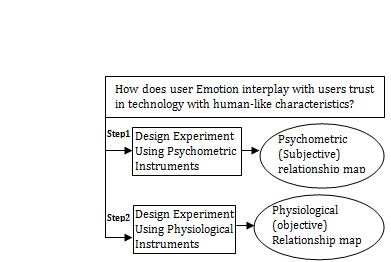
\includegraphics[width=0.5\textwidth]{maps}
    \caption{A picture of a gull.}
\end{figure}


\begin{enumerate}
    \item  The first experiment will employ psychometric instruments for collecting subjective data and evaluating the interplay between emotion and trust. Psychometric instruments are adopted from Gullathi et.al \cite{gulati2017modelling:twentysix}[26], GEW V2 \cite{scherer2005emotions:thirtysix},\cite{scherer2013grid:thirtyseven} and game interaction data.
    \item The second experiment will employ physiological sensing instrument for collecting physiological     data and analyzing the interplay between emotion and trust in technology with human-like characteristics. Physiological instruments are one or all  EEG, ECG, and GSR.
\end{enumerate}
In each experiment, we will use intelligent personal assistant known as Google assistant.
\section{Expected Contribution, Conclusion and Future Work }
\subsection Expected Result
This research  result is a conceptual mapping relationship between various emotional affect to trust (belief, intention, and behavior) in technology with human-like characteristics with both psychometric and physiological evidence. This will elicit and inform HCI practitioners. Designers, researchers and all stakeholder of future technologies (human-like technologies) on the effect emotional affect has on trust behavior, intention and belief so as to guide in development of human-like technologies that are highly persuasive and acceptable to user.
\subsection {Conclusion}
In conclusion, we have described the road map to a new era in understanding and sustaining the present and future technology as technology continues to evolve. Through understanding the interplay between the two common persuasive indicators to further understanding and enable the development of technological artifacts that can be persuasive to users and cause users to change behavior towards technology with human-like characteristics although this is work in progress
\subsection {Future Work}
Once the correlation between emotion and trust in technology with human-like characteristics is established, with both empirical and physiological evidence is found. Further research effort can be tailored towards examining the same topic in the following areas:
\begin{enumerate}
    \item Several other human-like technologies for further validation eg. Driverless vehicles etc.
    \item Cultura perception  of human like technologies
    \item Design guidelines for human-like technologies
\end{enumerate}
